\chapter{Developer Documentation}
This chapter outlines the details of the implementation of the TaleCraft framework along with the overall project structure. Our framework is developed using Unity version 2022.3.61f1 and is compatible with Unity Hub, which can be used to open and manage the project environment. All referenced files are provided in Attachment A for further inspection.

\section{Architecture}
The core of the project is found in the \verb|Assets/TaleCraft| directory. \verb|Assets| is the standard location in Unity for storing scripts, game assets, and other project resources, and the folder \verb|TaleCraft| is our custom folder. The contents are organized into several subfolders, each serving a specific purpose, as described in the sections that follow.

\begin{itemize}
    \item \textbf{Runtime}: This folder contains all scripts that are executed during the game’s runtime. The codebase is further organized into five distinct modules: \verb|Core|, \verb|CommandSystem|, \verb|DialogueSystem|, \verb|InventorySystem|, and \verb|WalkingSystem|. Each of these categories contains specific functionality of the framework.
    \item \textbf{Editor}: It includes scripts that extend or customize Unity Editor. These scripts are not executed at runtime. The folder structure within \verb|Editor| mirrors that of the \verb|Runtime| folder.
    \item \textbf{Prefabs}: This folder holds reusable prefab assets utilized throughout the framework.
    \item \textbf{Resources}: It contains various assets required by the framework, such as sprite images and Unity Style Sheets (USS), which define the visual styling of the UI components. 
    \item \textbf{Examples}: The \verb|Examples| folder includes two prototype projects that demonstrate practical applications of the TaleCraft framework. Each prototype features its own scene along with supporting assets, such as custom scripts, prefabs, fonts, and sprites that are specific to those demonstrations. 
\end{itemize}

In the rest of this chapter, we focus on classes located in the \verb|Runtime| and \verb|Editor| folders, as well as the relations between them. In Figure \ref{fig:TaleCraft}, we can see a simple diagram describing the five main groups the classes can be divided into, as well as the connections between them. These groups are the following: 
\begin{itemize}
    \item \textbf{Core} scripts implement key functionalities of the framework, which include Prefab Manager and Input Manager. This system is closely examined in Section \ref{Core}.
    \item The \textbf{Command System} manages the logic behind interactions for items in the inventory as well as those in the in-game world. It is referenced from the Input Manager in the Core group and more information can be found in Section \ref{CommandSystem}.
    \item The scripts in \textbf{Walking System} take care of creating polygons representing the walkable areas (in)accessible to the player as well as the generating of a graph described in Section \ref{Analysis:Graph}. The system also enables movement of characters, which needs to be called from Command System in order to move closer to the required spot upon clicking on it. The Walking System is further examined in Section \ref{Walkingystem}.
    \item  Dialogue scripts in the \textbf{Dialogue System} handle both user-facing and back-end aspects of the dialogue system, such as managing the editing of dialogue graphs through an interactive interface or the saving and loading of graph data. Additionally, some scripts control the runtime logic of the dialogue nodes during gameplay, including tasks such as hiding or revealing specific choice options, triggering events, and displaying the appropriate dialogue text above the corresponding characters. This system is largely separated from other systems except for the reference to variables and conditions from the Command System. We will look closely at the system in Section \ref{DialogueSystem}. 
    \item Finally, the \textbf{Inventory System} is practically completely separated from other systems. This helps the developer choose what type of inventory they want or if they even want one. It can be, however, referenced from through the Unity Inspector. Scripts included in the system are described in more detail in Section \ref{InventorySystem} .
\end{itemize}

\begin{figure}[H]
\centering
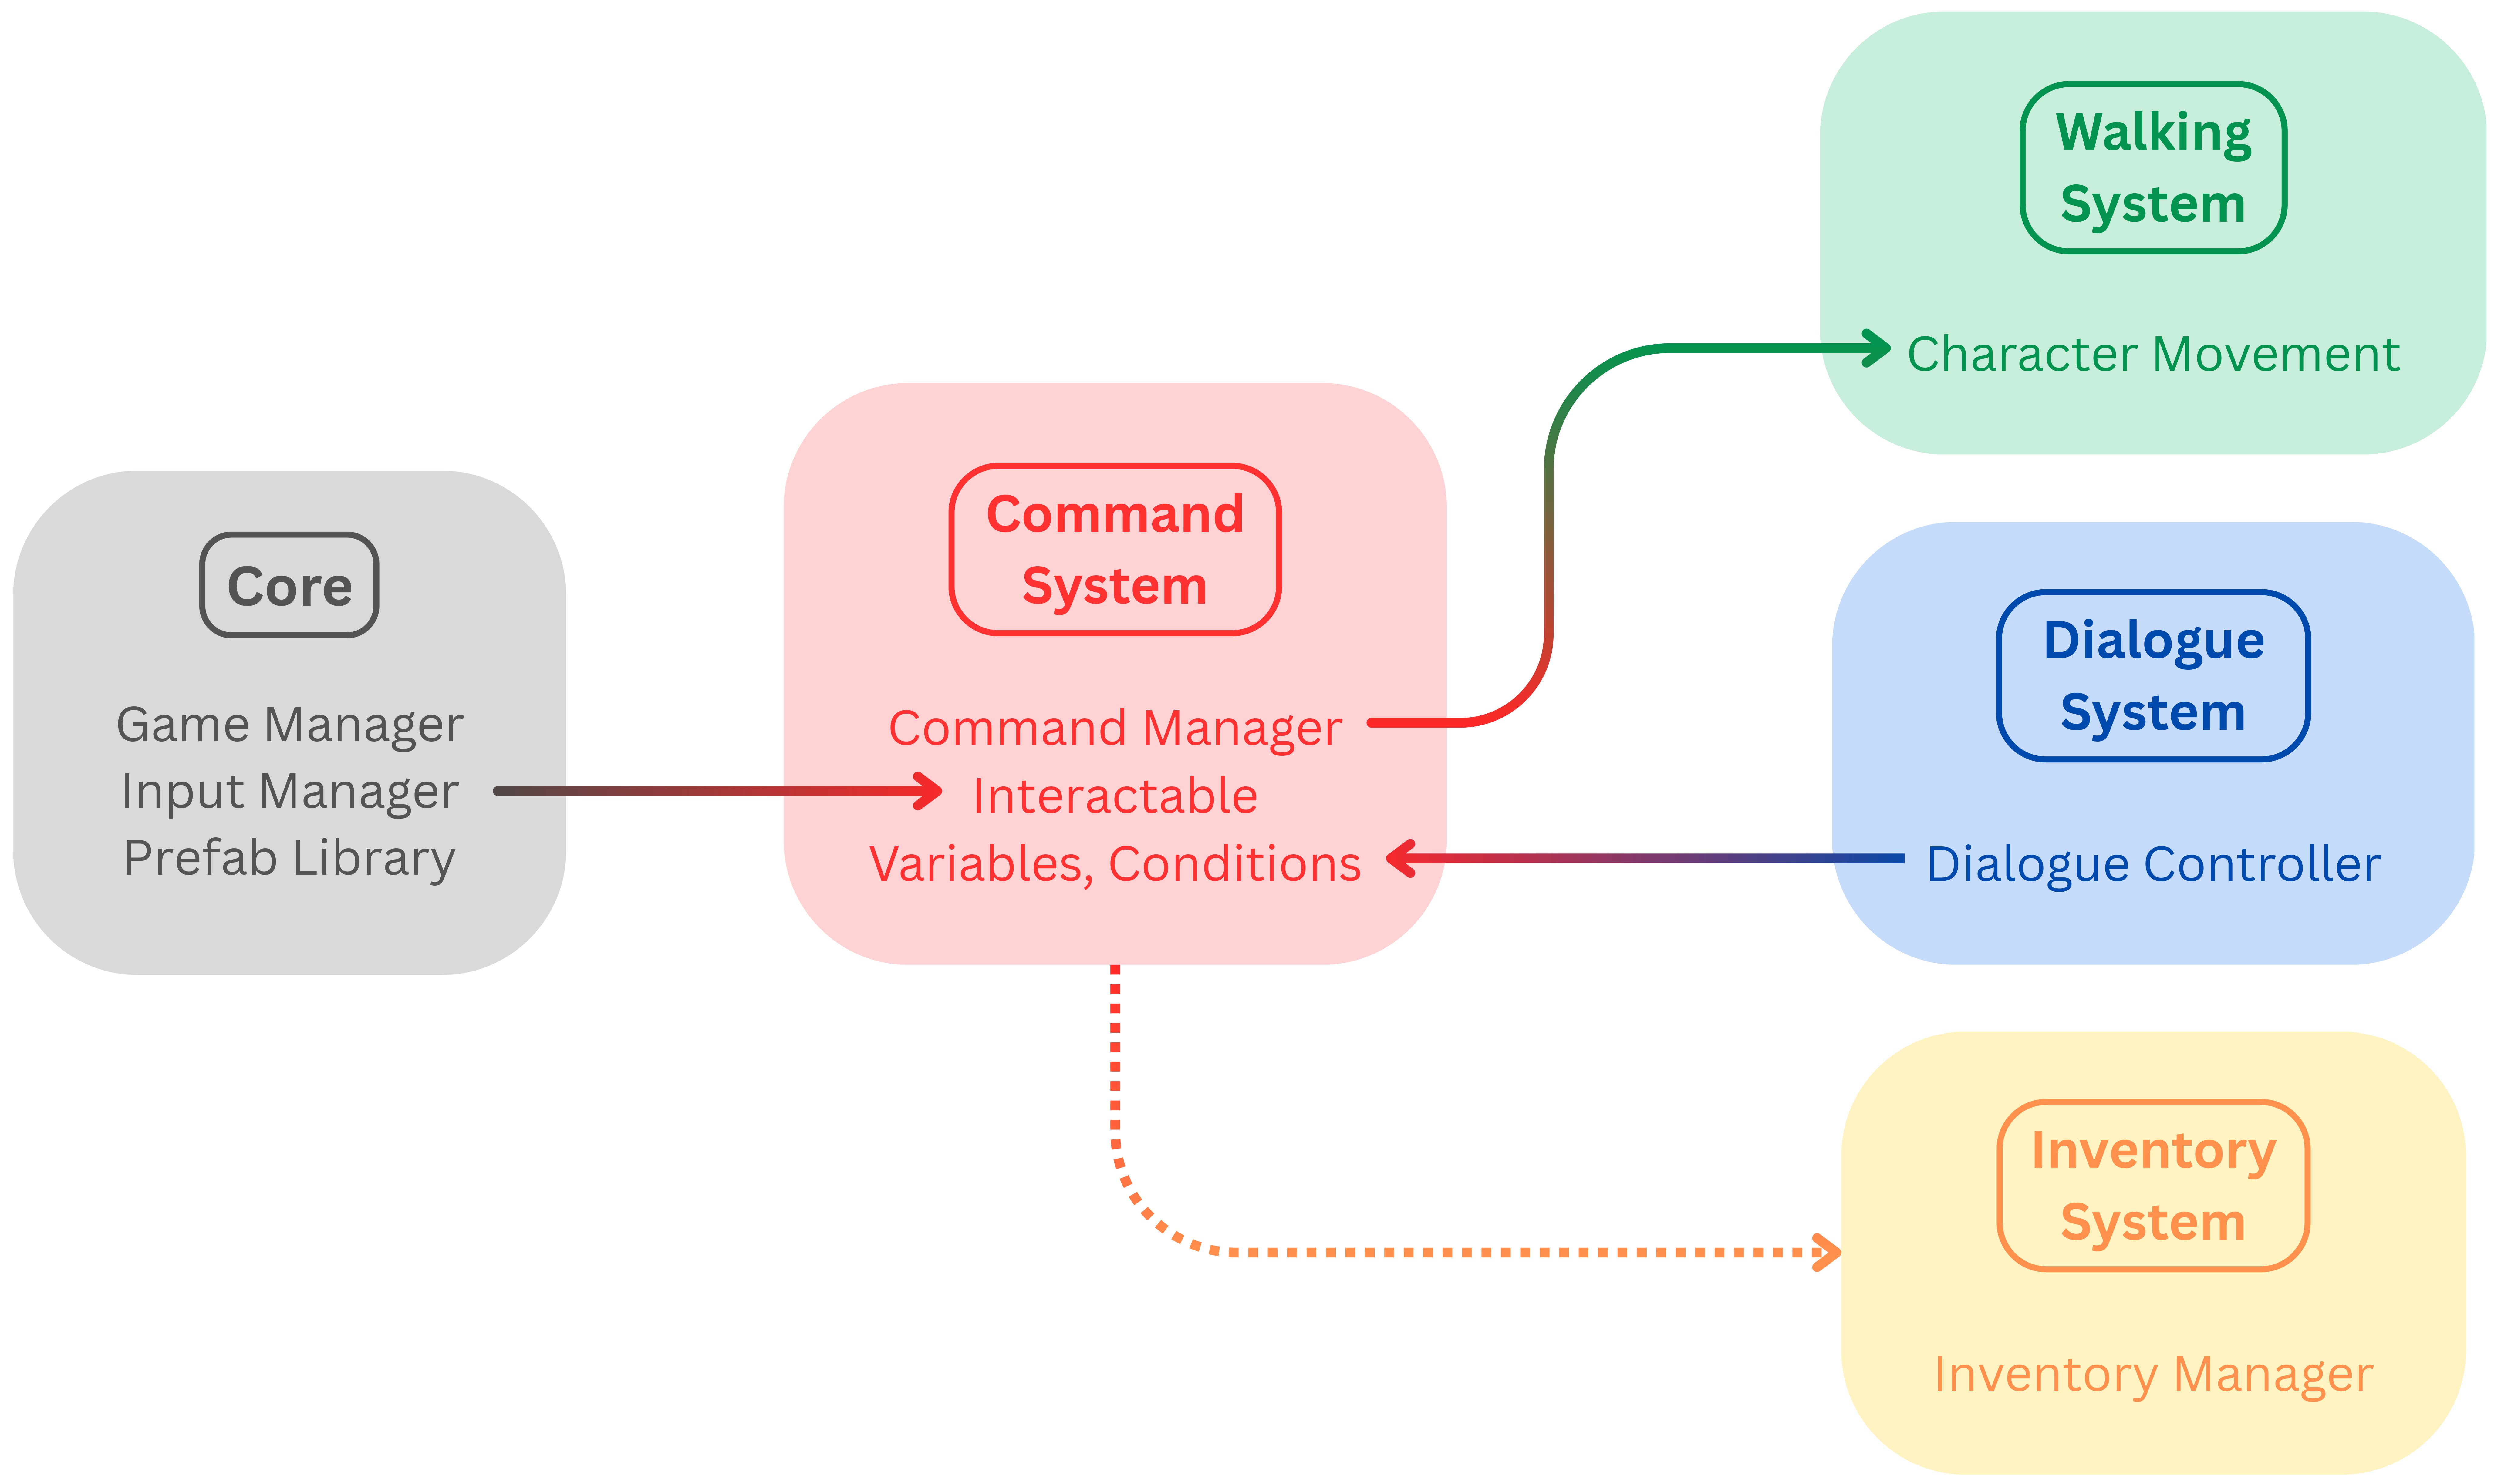
\includegraphics[width=0.85\linewidth]{img/framework_systems.png}
\caption{TaleCraft diagram.}
\label{fig:TaleCraft}
\end{figure}

\section{Core}
\label{Core}
The scripts in the \textbf{Core} folder work independently of one another and are responsible for managing foundational functionalities that fall outside the scope of the four main systems. 

\subsection{PrefabManager}
The \verb|PrefabManager| is a singleton that provides global access to shared systems. It holds a reference to the \verb|PrefabLibrary|, which stores prefabs used throughout the game. The singleton instance is created on demand by searching the scene, ensuring only one instance exists by destroying duplicates on \verb|Awake|. For now, it does not include many functionalities, but it can be useful to track gameplay-related logic.

\subsection{PrefabLibrary}
The \verb|PrefabLibrary| is a simple asset manager that stores references to named prefabs, making it easier for other scripts to access and spawn them without needing hardcoded links in the scene or code. It keeps a list of entries, each made up of a name and a corresponding \verb|GameObject|. The main method, \verb|GetPrefabByName|, looks up a prefab by its name and returns the matching object.

\subsection{InputManager}
The \verb|InputManager| listens for click input. When one occurs, it casts a 2D ray from the mouse position into the world. It also checks each hit collider for a \verb|WorldObject| component and calls its \verb|Interact| method, passing the world position and whether the left or right mouse button is pressed. If no \verb|Interactable| is found, it sends a move command to the player.

\section{Command System}
\label{CommandSystem}
The basis of \textbf{Command System} is built by \verb|CommandManager|, a script whose primary role is to hold commands used in the game. We also need to define objects the player can interact with, together with their behaviour.  Abstract class appropriately called \verb|Interactable| together with its inherited subclasses \verb|WorldObject| and \verb|InventoryObject| serve that purpose. In order to define suitable actions for each object in the scene, we need to set certain conditions. The classes \verb|Variable| and \verb|Condition| help with that by being able to determine simple logic and comparing variables. There are also two additional scripts that help with setting up the behaviour of \verb|InventoryObjects|, namely \verb|TriggerSetter| and \verb|SlotManager|.

\subsection{Variables}
The \verb|Variable| scripts define a system of variables, each based on a generic base class. They use \verb|ScriptableObjects|, so variables can be created as assets and shared across the framework. The core is the generic abstract class \verb|Variable<T>|, which stores a \verb|DefaultValue| (set in the inspector) and a \verb|RuntimeValue| (the current value used in the game). When the variable is enabled, it automatically resets \verb|RuntimeValue| to \verb|DefaultValue|. The class also provides methods to set or reset the value. Each concrete subclass specialises this for a specific type:

\begin{itemize}
    \item \textbf{BoolVariable} handles booleans and adds convenience methods to set true, set false, or flip the value.
    \item \textbf{IntVariable} handles integers and adds arithmetic operations like add, subtract, multiply, plus increment and decrement methods.
    \item \textbf{FloatVariable} works like IntVariable but for floats, supporting the same arithmetic and increment/decrement.
    \item \textbf{StringVariable} simply inherits from the generic base and does not add extra functionality since strings typically don't have arithmetic.
\end{itemize}

 \subsection{Conditions}
The \verb|Condition| classes provide a system for defining and evaluating various checks in the framework. At the core is an abstract base \verb|Condition| class that creates the common interface and functionality for all conditions. Building on this foundation, other subclasses handle specific data types such as boolean, integer, float, and string. Each of them compares the current runtime value of a variable with a target value to determine whether the condition is met: 

\begin{itemize}
    \item \textbf{BoolCondition} checks if a boolean variable matches an expected true or false value. It simply compares the variable’s current runtime value with the \verb|ExpectedValue| and returns true if they are equal.
    \item \textbf{IntCondition} checks an integer variable against an expected integer using one of several comparison operators (equal, not equal, greater than, less than, greater or equal, less or equal). The comparison to use is specified by the \verb|Comparison| enum. The \verb|Check| method runs the relevant comparison and returns whether the condition is met.
    \item \textbf{FloatCondition} works similarly to \verb|IntCondition|, but for float variables. It compares the current float value with an expected float using the same set of operators defined by the \verb|Comparison| enum.
    \item \textbf{StringCondition} checks whether a string variable’s current value exactly matches a specified expected string. It returns true if they are identical.
\end{itemize}

\subsection{Interactable}
The abstract class \verb|Interactable| serves as the main abstraction for any game object that the player can interact with in the TaleCraft system. It holds a list of \verb|CommandActions| that determine the behaviour of the object when certain conditions are met. 

The Figure \ref{fig:Interactable} describes the process of evaluating logic when a click is detected. When the player interacts with the object, the class first registers this interaction in the \verb|CommandManager|’s current sequence, linking the involved \verb|Item| and \verb|Interactable|. It then looks up the command that matches the currently selected command GUID in the \verb|CommandManager|. Before running the command, it checks whether the interaction sequence satisfies the command’s sentence structure rules (if those are enabled), which makes sure the player has interacted with the required number of objects. If everything checks out, the command execution includes moving the player closer to the target if the custom action demands it. Then, the class triggers the appropriate Unity events linked to that command action. If no matching custom action is found, it falls back to a default action defined by the \verb|CommandManager|.

\begin{figure}[H]
\centering
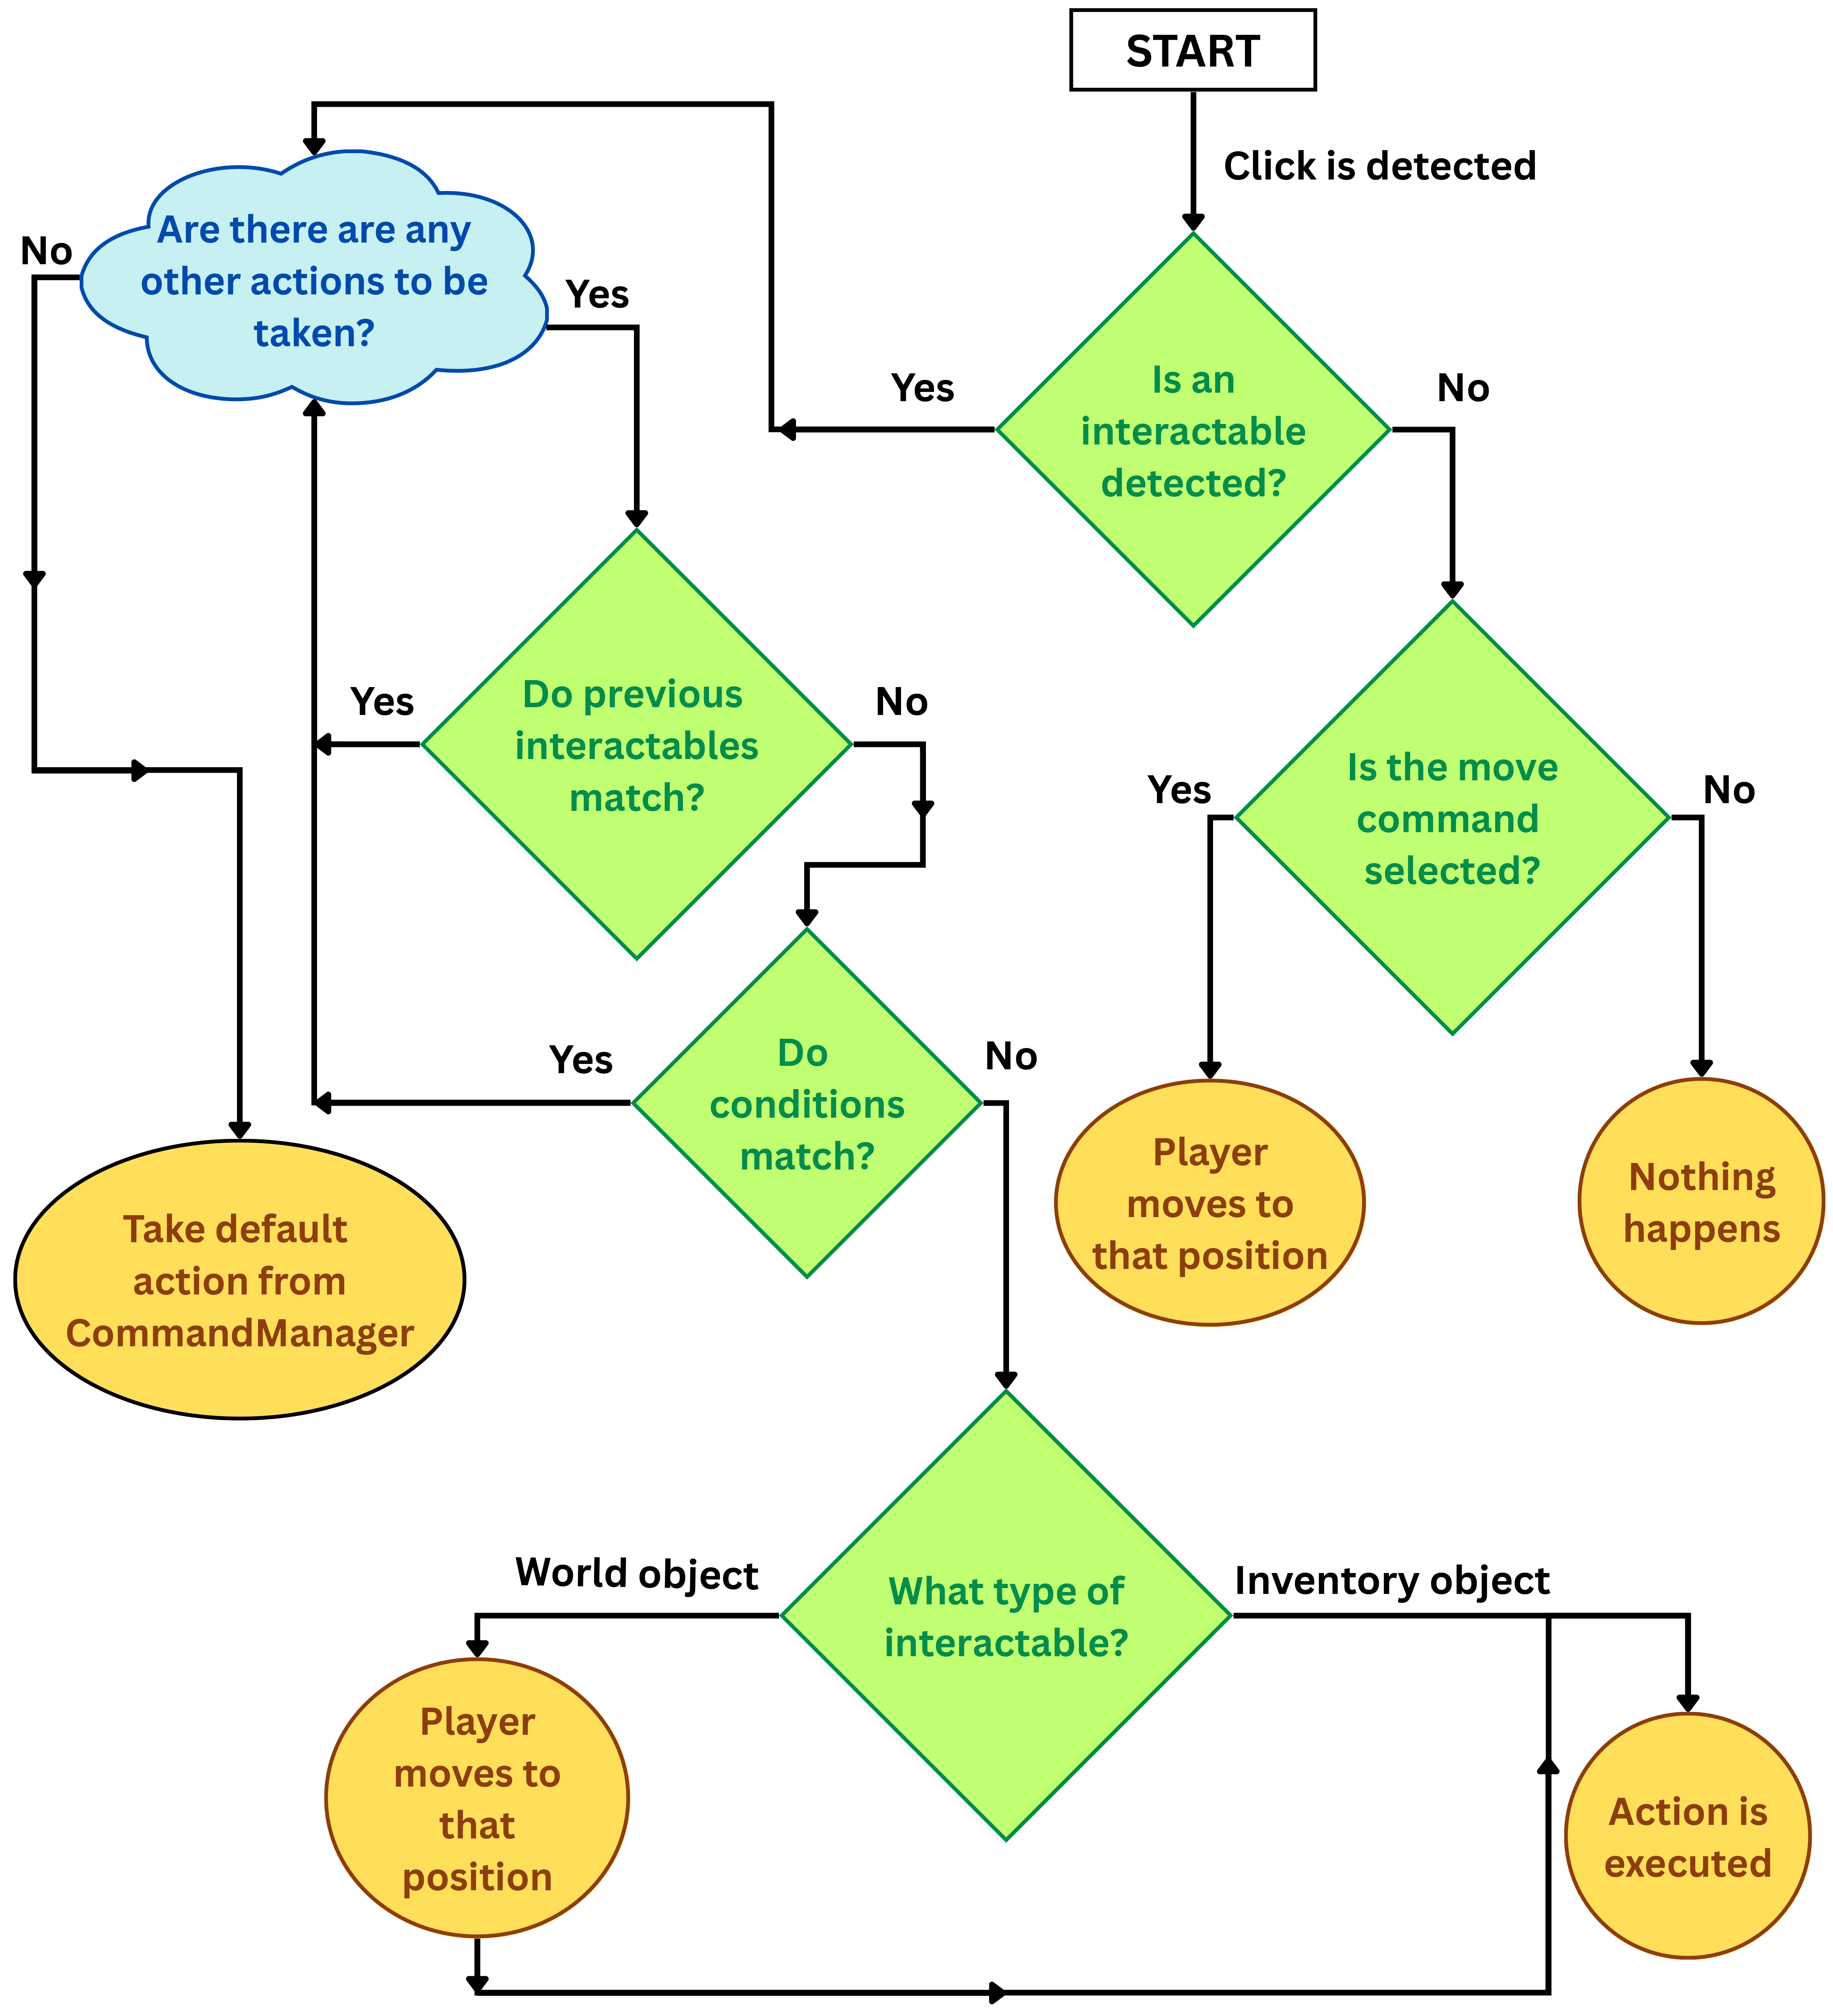
\includegraphics[width=0.9\linewidth]{img/Commands3.png}
\caption{Logic system.}
\label{fig:Interactable}
\end{figure}

\subsubsection{WorldObject}
\verb|WorldObject| extends \verb|Interactable| to represent interactable objects located in the game world, each linked to a \verb|WorldItem|. The class supports an array of \textit{go-to} points, which are positions the player can move to before interacting with the object. When executing a move-closer command, it calculates the shortest navigable path among these points and directs the player there. If no such point is found, it defaults to moving to the clicked position. The class also adds the option to display UI tags when the mouse cursor enters the object.

\subsubsection{InventoryObject}
\verb|InventoryObject| extends \verb|Interactable| to represent items held in the player’s inventory. Unlike other interactables in the game world, it does not work with world objects but with inventory slots instead. It retrieves command actions specific to the inventory item through the \verb|SlotManager|, which helps to reference items in the scene. 

\subsection{CommandManager}
The \verb|CommandManager| class is a singleton responsible for managing player commands, interaction sequences, and movement logic. It tracks three key commands \verb|selectedCommand|, \verb|defaultCommand|, and \verb|moveCommand|, which are stored as indices referencing a serialised list of \verb|CommandData|. Interaction sequences are stored in \verb|actionSequence|, which logs item-to-object interactions via \verb|ItemInteractablePair|. Temporary interaction data is kept in \verb|ActionTemp|, usually used when a mouse is hovering over an \verb|Interactable| object. The manager also supports basic grammatical validation of commands through \verb|setSentenceStructure| and a list of \verb|SentenceStructure| rules, which define valid object-connector sequences. Default or fallback actions are stored in \verb|DefaultActions|, a list of \verb|BasicCommandAction| objects that contain a reference to the command, a flag for movement behaviour, and a UnityEvent for triggering actions. These are synchronised with the command list through \verb|UpdateCommands()|.
 

%The \verb|CommandManager| is implemented as a singleton and serves as the central interface for managing game commands within the framework. Developers can create new commands directly through the editor interface by clicking the \textit{Add Command} button and assigning a name to the newly generated command. Commands can be renamed at any point during development; the system ensures that all references to the command across other scripts are automatically updated to reflect the new name. This feature significantly reduces the risk of broken references and allows developers to make adjustments even in later stages of the project without introducing inconsistencies.

%To assign both the movement command and the default command, the developer can simply select the desired options from a list of all available commands within the editor interface. They can also define rules that commands must adhere to, following the specifications outlined in Section \ref{Analysis:CommandStructure}. Additionally, the \verb|CommandManager| script allows assigning a default action for each command, which is executed when no other specific action is available.

\subsection{TriggerSetter}
The \verb|TriggerSetter| class manages interactive behaviour for inventory. It handles user input like hovering, clicking, and dragging, and links these actions to the appropriate inventory or command responses. Each instance is connected to an \verb|InventoryObject|, which allows it to connect behaviour to items in the player's inventory.

On startup, the class loads any required prefabs, such as the drag icon used during item movement, and sets up event listeners from \verb|CommandManager| to reset the UI when a command sequence ends. Mouse clicks on the slot trigger interactions are tied to the currently selected command, while hovering displays item details using shared UI elements to keep the interface clean and consistent. When the player begins dragging an item, a drag icon is created as a copy of the current inventory slot. This icon visually follows the mouse, while raycasts constantly check for valid drop targets underneath, such as another inventory slot or a world object. If the item is dropped on another \verb|Interactable|, the object’s \verb|Interact()| method is called. If no valid target is found, the command is cancelled.

\subsection{SlotManager}
The framework must be able to let users define the behaviour when inventory items interact with other items. It is not possible to define these actions in the instances of the items themselves, as doing so would be very difficult when crossing to other Unity scenes, since we can only reference \verb|GameObjects| of inventory items he \verb|SlotManager| holds a collection of \verb|Slot| instances, each pairing an \verb|InventoryItem| with its possible command actions.

A \verb|Slot| class links a single inventory item to a list of \verb|CommandActions|, which represent individual commands a player can use with that item. Each \verb|CommandActions| contains a reference to \verb|CommandData| (defining the command’s ID and name) and a list of \verb|LabeledAction|s. These labelled actions wrap a \verb|CustomAction| with a descriptive label, which link an action to a meaningful human-readable name.

\verb|CustomAction| holds the execution details for a command: it can require \verb|Interactables|, track previous ones, and check custom conditions before running. It also manages separate UnityEvents for left and right mouse clicks, with options to move the player closer during the interaction and duplicate actions across click types.


\subsection{Action Drawer and Window}
To organise the commands, we use the classes \verb|LabeledActionListDrawer| and \verb|ActionEditorWindow|. The \verb|LabeledActionListDrawer| is a utility designed to make it easier to manage a list of \verb|LabeledActions| directly in the Inspector. The \verb|Initialize()| method sets up \verb|ReorderableList|, including custom drawing behaviour for each item. Each entry in the list includes an option to open a separate \verb|ActionEditorWindow| for modifying the action’s configuration. This class is a custom Unity \verb|EditorWindow| designed to provide a user-friendly interface for editing \verb|LabeledAction| objects in Inspector. When launched via the static \verb|Open()| method, the window shows collapsible sections for different components of the action. These include a list of \textit{Previous Interactables} (other objects this action may rely on), a list of editable \textit{Conditions}, and settings for mouse button triggers.

The \textit{Previous Interactables} list contains all \verb|Interactables| that are required to have been interacted with in order to execute this action. \textit{Conditions} can be added dynamically using a context menu that finds all non-abstract subclasses of \verb|Condition| via reflection. Finally, the window allows editing separate action lists for left and right mouse buttons. If the \verb|DuplicateActions| option is enabled, however, the editor shows a shared list of actions for both mouse clicks. 

\subsection{DisplayCommands}
The \verb|DisplayCommands| class is responsible for managing the visual layout and behaviour of command buttons in the Unity UI. It keeps track of the currently active commands and also stores any commands from the global \verb|CommandManager| that are not currently shown. 

On startup, it sets up the buttons by assigning each one a name and hooking up a click listener that selects the corresponding command using its GUID. The button labels are set through the \verb|ApplyCommandNames()| method, which looks up the name of the linked \verb|CommandData|. The \verb|ReloadUnused()| method checks for commands that exist globally but are not in the current UI and stores them separately for possible future use. To keep the interface clean, \verb|RemoveChildren()| deletes buttons that no longer match a valid command. If the command name changes, \verb|ReloadUIName()| updates the button label. Button clicks are set through \verb|SetClick()|, which connects each button to the global command selection logic. Finally, \verb|GetPosition()| calculates the placement of each button on the grid based on layout parameters such as spacing, column count, and offset.

 \subsection{DisplaySentence}
In Section \ref{ActionPanel}, we decided to implement a sentence that indicates the current sequence of actions for the player. The \verb|DisplaySentence| class handles rendering a sentence in the UI and updates dynamically based on the currently selected command and its sentence structure (defined in the \verb|CommandManager|). During each frame, it checks if the text component is valid and updates its content using the \verb|GetSentence()| method. If \verb|onMouse| is enabled, the sentence display is also repositioned to follow the mouse, offset by the \verb|shiftBy| value.

The sentence is built using the \verb|SentenceStructure()| of the selected command. It always begins with the command’s base name and then adds other elements according to a list of rules. These rules define whether each part of the sentence should be a connector (like a keyword) or an object (like an item or interactable).

If a rule calls for a connector and one is available, it is inserted into the sentence. If it expects an object and one is present in the current \verb|ActionSequence|, it uses the object's name. If no object is available, but there is a temporary action, it uses that instead and stops the sentence there.


\section{Walking System}
\label{Walkingystem}
The primary part of \textbf{Walking System} (described in Figure \ref{fig:WalkingSys}) is the class \verb|WalkingMap|. The project a prefab which contains a GameObject with the \verb|WalkingMap| as a component. The prefab also comes along with a \verb|Polygon| that defines the walkable area of the game. The \verb|WalkingMap| manages the collection of polygons that represent where characters are allowed to move. Class\verb|WalkingSystem| generates an instance of the prefab into the scene via a custom menu option.
The next important part of the system is class \verb|PathFinder|, which determines how a character should navigate from one point to another by calculating the paths through a graph structure. The graph is represented by class \verb|Graph|, which consists of \verb|GraphNodes| and \verb|GraphEdges| that are set based on the geometry of the walkable area. The class \verb|CharacterMovement| then uses the paths created by \verb|PathFinder| to move characters around the scene. Finally, \verb|SpriteScaler| dynamically adjusts the visual scale of the character based on the position on the map, giving the illusion of depth. Together, these components form the complete walking system used in TaleCraft.


\begin{figure}[H]
\centering
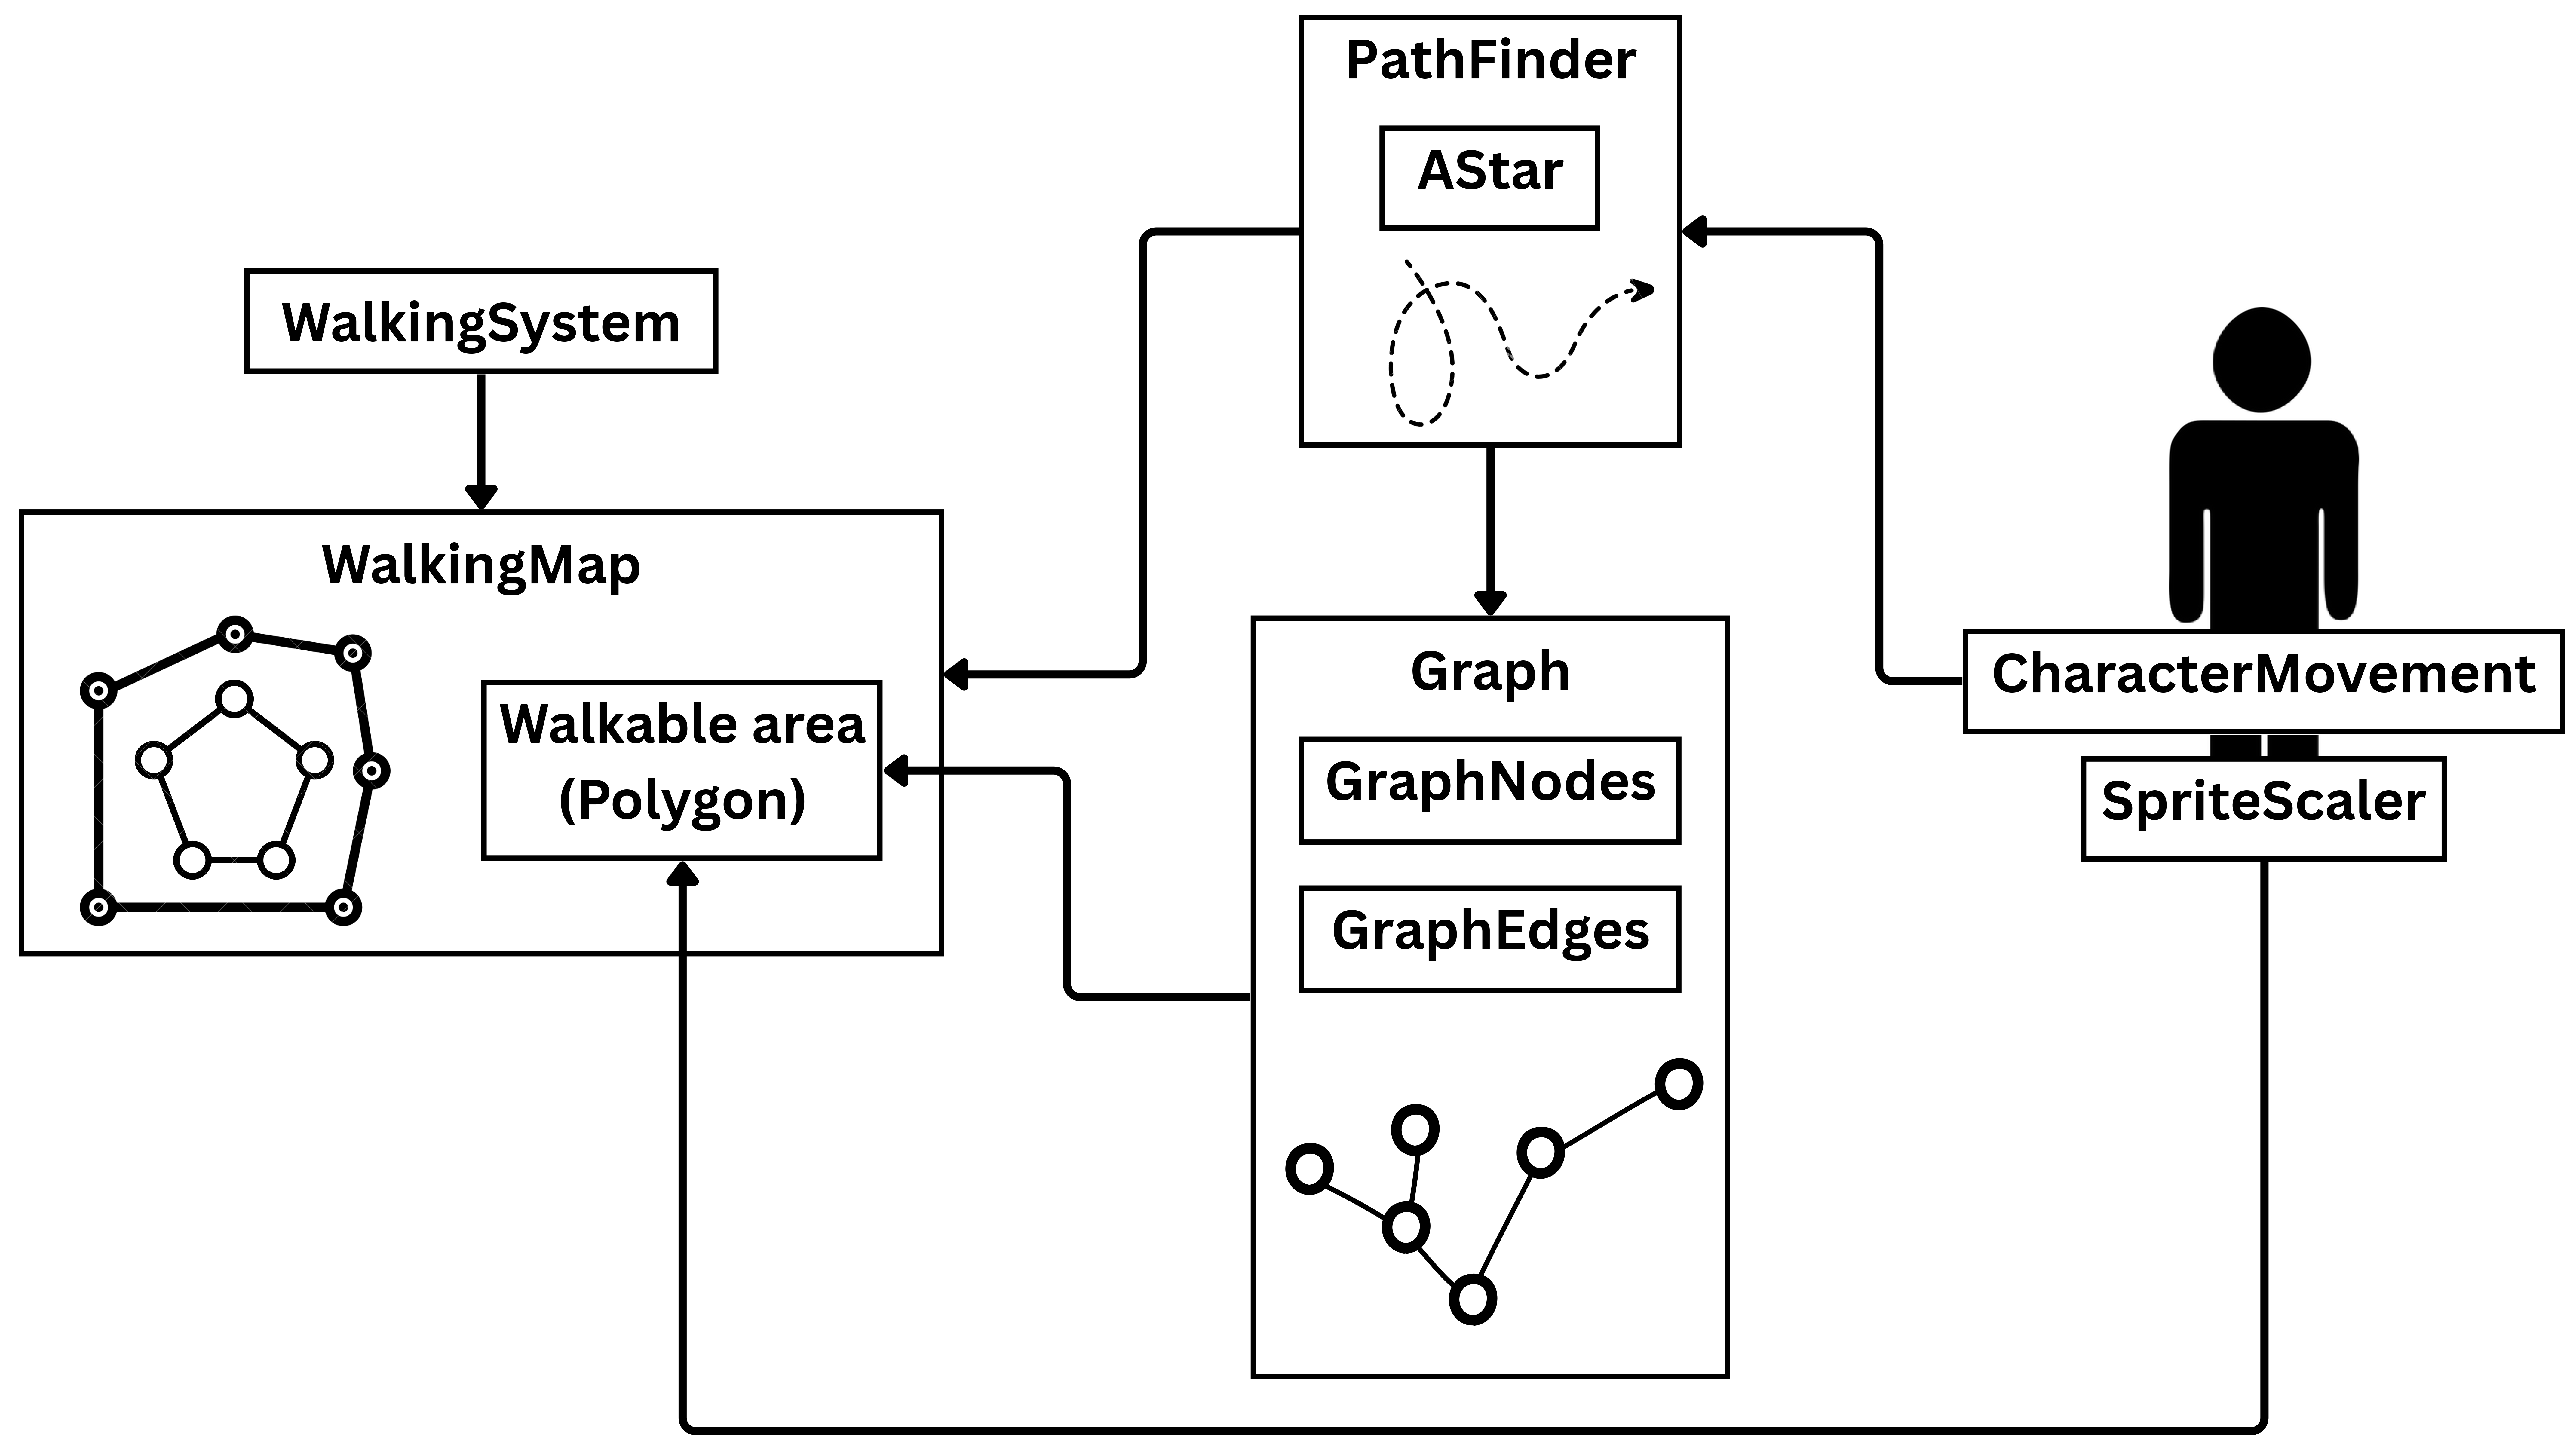
\includegraphics[width=0.85\linewidth]{img/Walking2.png}
\caption{Walking system.}
\label{fig:WalkingSys}
\end{figure}

 
\subsection{Polygon}
In Section \ref{Analysis:Polygon}, we decided to represent the walkable area as well as the obstacles in form of polygons, so let us have a look at its implementation. The \verb|Polygon| class defines a collection of connected points (\verb|GraphNode|s) that form a polygon in a 2D space. It is designed to run both during gameplay and in the Unity Editor, where it dynamically manages and visualises its vertices using Gizmos. The class ensures that the vertices are ordered clockwise for correct algorithmic behaviour, which is validated by the \verb|IsOrientationClockwise()| method.

To assist in pathfinding and calculations, \verb|Polygon| includes methods to determine whether a point lies inside the shape, whether a point should be removed from the polygon, and where the nearest point on the polygon's edge is relative to a given location. These checks are based on geometrical principles such as ray-casting and distance-to-segment calculations. In edit mode, the polygon continuously scans its child objects to update its list of vertices using the \verb|ListChildrenWithComponent()| method. It expects these children to have a \verb|Point| component and uses their positions to form the polygon.

Graphical properties like edge drawing, point visibility, and point scaling are configurable and updated automatically. The editor visualisation adapts to zoom using Unity’s handle size system to maintain consistent point sizes when viewing in the Scene window.


\subsection{Graph}
\verb|Graph| class models a cyclic, undirected graph composed of \verb|GraphNode| vertices and \verb|GraphEdge| connections. It is the foundational data structure used in pathfinding, as established in Section \ref{Analysis:Graph}. Each node is stored in a list, and its neighbours are tracked in a parallel adjacency list. Edges between nodes are recorded in a dictionary, keyed by the smaller of the two node indices, making sure that we get an undirected and non-redundant representation.

The graph provides utility functions for calculating Euclidean distances between nodes and between a point and a line segment, which are essential for visibility checks and path optimisation. Nodes and edges can be dynamically added. When an edge is added, it is also registered in the neighbour lists of both nodes to maintain symmetry. The graph keeps references to a \verb|Start| and \verb|End| node, which are required for executing the pathfinding algorithm.

 A \verb|GraphNode| encapsulates a 2D coordinate and an optional reference to a \verb|Point| game object. It serves as a vertex in the \verb|Graph|. Nodes can be constructed from Unity \verb|Vector3|, raw coordinates, or \verb|Point| objects. The node exposes its position through \verb|X|, \verb|Y|, and a \verb|GetLocation()| method that returns a \verb|Vector2|.

 A \verb|GraphEdge| represents an undirected connection between two graph nodes, identified by their indices and storing a precomputed length for efficiency. The edges are normalised such that the smaller node index is always \verb|N1|, which standardises storage and retrieval in \verb|Graph|.


\subsection{PathFinder}
\verb|PathFinder| is responsible for calculating the shortest navigable route between two points within the walkable area defined by \verb|WalkableMap|. It constructs a visibility graph based on polygonal data and uses A* search to determine the optimal path.

The core logic starts by constructing a graph in which nodes are placed at concave vertices of the defined walkable area and obstacle polygons. Additional nodes are inserted at the given start and end positions, which can be adjusted to meet constraints, such as staying inside the main polygon or outside obstacles, depending on the settings of \verb|WalkableMap|.

To determine possible connections between nodes, \verb|PathFinder| uses line-of-sight (LOS) checks. These ensure that no segment intersects any polygon edge and that the midpoint of each connection lies within the walkable region and outside obstacles. Nodes that satisfy the LOS criteria are connected with graph edges. The shortest path is then computed using an A* algorithm in the \verb|AStar| script applying a Euclidean heuristic function.  The resulting path consists of a list of \verb|GraphNode| points and their respective distances. For visualisation purposes, the class can draw both the full graph and the shortest path using Unity Gizmos.


% \subsection{AStar}
%The \verb|AStar| class implements the A* search algorithm to compute the shortest path between two nodes within a \verb|Graph| object. It uses a best-first search strategy, implementing a cost function \verb|f(n) = g(n) + h(n)|, where \verb|g(n)| is the known cost from the start node to node \verb|n|, and \verb|h(n)| is a heuristic estimation of the cost from \verb|n| to the goal. The heuristic is based on Euclidean distance, ensuring admissibility and consistency for this geometric use case. Finally, upon reaching the goal, a backtracking method (\verb|ConstructPath|) reconstructs the optimal path. 


\subsection{SpriteScaler}
In order to simulate depth and give characters the appearance of existing in 3D space (as discussed in Section \ref{analysis:depth:scaling}), the \verb|SpriteScaler| class dynamically adjusts the scale of a \verb|GameObject| based on its position.  The scale is continuously updated during both runtime and edit mode using the \verb|[ExecuteAlways]| attribute. This makes sure that the object's size always matches its intended perspective in the scene. Having the correct scale during editing is especially useful when setting up the layout before running the game. The script supports multiple scaling modes including none, X-axis-based, Y-axis-based, and a custom scale blending based on proximity to vertices of a defined polygonal walkable area.

Using configurable parameters such as \verb|upperScale|, \verb|lowerScale|, and \verb|perspectiveFactor|, the first two modes (X-axis / Y-axis scaling)  calculate the appropriate scale by interpolating the object's position relative to the walkable polygon’s bounds. The custom scaling mode, on the other hand, employs a weighted average of vertex scales that is inversely proportional to their distance. 


\subsection{CharacterMovement}
The \verb|CharacterMovement| class manages the movement itself. It integrates with a \verb|WalkableMap| and a pathfinding system (\verb|PathFinder|) to compute traversable paths between points. Movement allows the character to smoothly interpolate along a computed path using coroutines while adapting the speed based on the object's scale via the \verb|SpriteScaler| component. The \verb|Move| methods handle both direct target positions and precomputed paths, initiating a coroutine that interpolates the character’s position over time. The class also ensures that if a new movement command is issued mid-transition, the current motion is halted, and a new path is followed. It also supports visual debugging via Unity’s Gizmos for path visualisation.

 
\subsection{WalkableMap}
Everything comes together in \verb|WalkableMap|, which manages the pathfinding logic within a scene by maintaining and organising the walkable area and a collection of obstacles. It is responsible for ensuring that the start and end points of a path remain within valid constraints, such as staying inside the main walkable polygon or outside defined obstacles.

The script is initialised by identifying all child objects tagged as obstacles and storing their corresponding \verb|Polygon| components. These obstacle polygons, along with the main walkable polygon, are used to construct a map for navigation. Any null references within the obstacle list are actively removed to maintain consistency. \verb|WalkableMap| also provides options to visualise the graph's structure and the calculated path in the editor using specified colors from the inspector.

\subsection{WalkingSystem}
The \verb|WalkingSystem| script provides editor functionality to instantiate a predefined walking system prefab into the current Unity scene. It integrates into the Unity Editor menu and allows developers to quickly add the walking system via a custom menu item. After clicking on the option, the script finds the corresponding prefab from a centralised \verb|PrefabLibrary|, and instantiates it in the hierarchy.


\section{Inventory System}
\label{InventorySystem}
The Inventory System consists of three main components: a way to represent items within the framework (the \verb|Item| class, discussed in Section \ref{Items}); a manager that keeps track of the inventory’s contents (\verb|InventoryManager|, detailed in Section \ref{InventoryManager}); and a UI component that visually displays the inventory (\verb|DisplayInventory|, covered in Section \ref{DisplayInventory}). 

\subsection{Items}
\label{Items}
The \verb|Item| script and its subclasses define the different item types used in TaleCraft’s inventory system. They take advantage of Unity’s \verb|ScriptableObject| to make managing and saving item data easier.

At the base is the \verb|Item| class, which stores basic information, such as the item’s name and description. It also includes a simple method to rename the item when needed.

The \verb|InventoryItem| class inherits from \verb|Item| and adds data for how the item should appear in the UI. This includes an \verb|ItemImage| that holds a sprite and a color. The \verb|ApplyTo()| method lets us apply this image data to a Unity UI Image component, ensuring that the item is displayed correctly in the inventory. \verb|ItemImage| is a straightforward container for the sprite.

Lastly, \verb|WorldItem| is another subclass of \verb|Item| meant for items that exist in the game world but might not be carried by the player. It does not add extra features but serves to clearly separate world objects from inventory items for game logic purposes.
 
\subsection{InventoryManager}
\label{InventoryManager}
The \verb|InventoryManager| class provides a basic inventory system using a list to keep track of a collection of \verb|InventoryItem| objects. It also supports adding new items, removing existing ones, and clearing everything from the inventory. Whenever the inventory changes, it fires an event to let any connected systems know about the update. The \verb|RestrictSize| flag determines whether the inventory should enforce a size limit, which is set by the \verb|MaxSize| value.

When adding an item, the manager first checks two things: whether the inventory has reached its size limit (if size restrictions are turned on), and whether the item is already in the list. If both checks pass, the item is added and the change event is triggered. Removing an item simply tries to take it out of the list. If the item was found and successfully removed, the event is triggered to reflect the update. The \verb|ClearInventory()| method just empties the list completely and notifies any listeners that the inventory has changed.

\subsection{DisplayInventory}
\label{DisplayInventory}
When it comes to displaying the inventory to the player through the UI, the class \verb|DisplayInventory| is responsible for it. It works together with the \verb|InventoryManager| to stay in sync with the actual inventory data and updates the visual elements whenever changes occur. At the beginning, it configures things like slot size, scaling, and layout logic. During initialisation, it also looks for a child \verb|GameObject| named \verb|"Items"|. If it does not exist, the script creates it to serve as the container for all item slots. Right after that, it triggers a UI refresh to display the current inventory.

To update the UI, the script either clears or reuses existing slot \verb|GameObjects| to match the number of items in the inventory. For each item, it reuses a slot if one is available, or instantiates a new one from a prefab. Then it fills in the visual content of the slot with the data of the item.

The class supports two display modes: one that shows only the item's icon and one that shows only its name. In both cases, items are arranged using a grid system that calculates each slot’s position based on its index and the total number of columns. To manage larger inventories, only a portion of the items are visible at a time, limited by \verb|MaxItemCount| and controlled using the \verb|ItemIdx| offset. Any items outside this visible range are hidden, and the grid layout is recalculated every time something in the inventory changes.
 
\subsubsection{InventoryScrollButton}
\verb|InventoryScrollButton| manages a scroll button within the inventory UI, allowing users to navigate through a list of items. Depending on its configuration, the button shifts the view either forward or backward and updates the item display accordingly. During initialisation, the component saves the button's default image color for later use in visual feedback. When the component is enabled or disabled, it subscribes or unsubscribes from inventory change events to ensure the button stays visually consistent with the current inventory state.

The \verb|SetColor()| method updates the button’s appearance based on whether scrolling is currently possible. If the inventory has reached the beginning or end, the button is visually dimmed using a predefined inactive color to indicate that further scrolling in that direction is not available. When clicked, the \verb|Scroll()| method modifies the \verb|ItemIdx| value that defines the starting index of visible items in the inventory. It then iterates through the inventory’s UI elements, updating their visibility and position so that only the currently relevant items are shown.


\section{Dialogue System}
\label{DialogueSystem}
Let us move onto the implementation of the dialogue system. The centrepiece of the visualisation of the dialogue is class \verb|DialogueGraphView| (\ref{devlog:DialogueGraphView}), which uses the main features of the \verb|GraphView| API and displays them using \verb|DialogueWindowEditor| (\ref{devlog:DialogueWindowEditor}). The window then uses elements (\ref{devlog:Elements}) from the API such as nodes, edges and groups to represent a dialogue graph. This is, however, only done through Unity Editor, which means that we cannot access the data during runtime. To solve this, we define \verb|DialogueGraphData| (\ref{devlog:DialogueGraphData}), which stores the values of the elements of the graph together with the relationships between these elements. The final piece of the graph management is a saving and loading system intuitively called \verb|DialogueSaveLoad| (\ref{devlog:DialogueSaveLoad}), which serves as a bridge between \verb|DialogueGraphData| and the actual graph in \verb|DialogueWindowEditor|. Now, we are left with \verb|DialogueController| and \verb|DialogueUIController| (\ref{devlog:DialogueController}, \ref{devlog:Dialogue UI}), which manage the logic of traversing the data nodes of \verb|DialogueGraphData| followed by displaying the appropriate UI on the screen. In the following sections, we examine the actual implementations of these classes.

\subsection{Elements}
\label{devlog:Elements}
A graph consists of nodes, edges, and, in our case, also groups (see Section \ref{Analysis:Dialogue:Features}). While Unity’s \verb|GraphView| API provides built-in support for these elements, their default implementations are too minimal for our needs. To support features like saving, loading, and conditional branching, we must extend these base components with additional properties. One such property is a globally unique identifier (GUID), which allows us to maintain reliable references to nodes and groups across editing and serialization. In this framework, each node and group is assigned a GUID to support consistent tracking. Edges are defined by the connections between nodes and this relationship can be stored directly within the nodes themselves. Therefore, the following section will closely examine the extended implementations of nodes and groups.


\subsubsection{Nodes}
The nodes are a central piece of the dialogue graph. It consists of various types of nodes.

At the heart of this system is \verb|BaseNode|, which inherits from the \verb|Node| in \verb|GraphView| API and provides all shared behaviour for node-based interaction. It handles input/output port creation, holds a unique identifier, and manages condition logic such as booleans, integers, floats, and strings. These conditions are used to control the flow of the dialogue graph based on variables, and the node provides a dynamic UI to configure them. It manages a \textit{Visited} flag, which can be toggled or generated as a \verb|Variable|. All of the other nodes inherit from the \verb|BaseNode| all of the properties as well as the methods.

\verb|StartNode| represents the entry point of a dialogue flow. It is a minimal extension of \verb|BaseNode|, featuring a single output port and simple setup for ID and visited state. This node effectively serves as the beginning of the conversation graph, initiating the traversal through the dialogue nodes.

 The \verb|DialogueNode|, on the other hand, represents a standard dialogue step in the graph. It contains one input port and multiple output ports for branching conversations, that can only be connected to a \verb|ChoiceNode|. Internally, it holds a list of text boxes where each entry can represent a character's line. It supports two dialogue continuation styles: automatic after a wait time, or manual via player input. The visual elements dynamically adjust based on the continuation type and presence of choice ports. Choices are represented by additional output ports and are stored in \verb|DialogueNodePort| instances.

 The \verb|ChoiceNode| is designed for player decision points. It displays a single text field and conditions that determine whether it appears or not. The node includes one input port and one output port. All conditions are inherited from the base node system and are managed using the overridden methods \verb|AddCondition|.

\verb|BranchNode| extends \verb|BaseNode| to implement decision-making logic. It sets up one input port and two output ports labelled \textit{True} and \textit{False}, allowing the dialogue to split based on the evaluation of its conditions. 

Using \verb|EventScriptableObject|, the \verb|EventNode| allows triggering events assets. These objects reference \verb|DialogueEvent| assets that encapsulate game-side logic. Each event is shown in the UI as an \verb|ObjectField| and can be added or removed with the corresponding buttons. All event assets are stored in a list and serialised through the node class.

Finally, \verb|EndNode| signals the end of a dialogue path. It contains only one multi-input port and no output ports. Internally, it uses an \verb|EnumField| to define how the dialogue ends (exit, return to the start, or repeat the last node). 
 

\subsubsection{Groups}
As established in Section \ref{Analysis:Dialogue:Features}, we would like to have the ability to organise subsets of nodes within the graph, and the \verb|BaseGroup| class serves that purpose. It is a lightweight extension of Unity’s \verb|Group| from the \verb|GraphView| system, used in the Unity Editor for grouping nodes visually in a graph interface. It adds a single field, \verb|GroupGuid|, which uniquely identifies the group via a generated GUID. This is useful for saving, loading, and tracking groups independently of their visual layout.


\subsection{DialogueGraphData}
\label{devlog:DialogueGraphData}
In order to access dialogue graphs during the gameplay, we, of course, need a way to represent the data. The \verb|DialogueGraphData| class functions as a data container for the dialogue system. Implemented as a \verb|ScriptableObject|, it exists as a persistent asset that can be saved, edited, and reused directly in the Unity Editor. Its primary responsibility is to store the entire structure of a dialogue graph, including dialogue lines, choices, branching logic, events, and the connections between nodes.

All node data inherit from the \verb|BaseNodeData| class, which provides common properties such as a unique identifier (GUID), editor position, display name, a runtime \verb|Visited| flag, and a collection of conditions. More specialised node types include \verb|DialogueNodeData| (storing character-linked dialogue text), \verb|ChoiceNodeData| (for player-selectable options), \verb|EventNodeData| (triggering scripted actions), \verb|BranchNodeData| (evaluating conditions), and \verb|EndNodeData| (defining how the dialogue branch concludes).

In addition to node data, the class stores group and edge information. \verb|GroupData| allows developers to visually organise related nodes within the editor by assigning them to named movable containers. Each group includes an ID, a name, a position in the graph view, and a list of GUIDs corresponding to the nodes it contains. \verb|EdgeData| defines the directional links between nodes and represents the logical flow of the conversation. Each edge stores the GUIDs and port names of both the source and target nodes, allowing the system to determine the next node in the sequence during both editing and runtime.


\subsection{DialogueSaveLoad}
\label{devlog:DialogueSaveLoad}
The saving and loading of a graph occurs in the \verb|DialogueSaveLoad| class. It is achieved by serialisation and deserialisation of the data the graphs consist of. When saving, the class converts the current graph state into an asset \verb|DialogueGraphData|. This process involves capturing the structure and properties of groups (name, position, and contained nodes), serializing connections between nodes, and storing the data specific to each node type. For example, \verb|Dialogue Nodes| store text box content and port configurations, \verb|Event Nodes| preserve references to \verb|ScriptableObject| instances, and \verb|Branch Nodes| save conditional data as well as the GUIDs of the nodes connected to their \textit{True} and \textit{False} outputs.

During loading, the class first clears the current graph to ensure a clean state. Then it reconstructs groups based on the stored data, followed by instantiating nodes using their saved attributes such as position, GUID, \textit{Visited} status, and type-specific data. The nodes are then reassigned to their appropriate groups, and the edges are reconnected by matching saved port names with the correct input and output ports.


\subsection{DialogueGraphView}
\label{devlog:DialogueGraphView}
\verb|DialogueGraphView| inherits from Unity's \verb|Experimental.GraphView| and manages the visual interface and logic of a node-based dialogue system. It supports creation, manipulation, serialization, and deserialization of various dialogue nodes and groups within the editor. The class also enables standard manipulations such as dragging, selection, and zooming and includes a customizable minimap for navigation. Users can interact with the graph by adding nodes via a search window, grouping them, or copying/pasting selected elements. 

For copy-paste functionality, the script serializes selected nodes, edges, and groups into a \verb|CopyData| class, which regenerates them at the mouse position after pasting. During serialization, each node is assigned a new GUID and edges are reconstructed by mapping these new GUIDs. The grouping is preserved by reassigning nodes into their respective regenerated groups.

 
\subsection{DialogueWindowEditor}
\label{devlog:DialogueWindowEditor}
The \verb|DialogueWindowEditor| class is a custom Unity Editor window that is used to create and edit dialogue graphs. It is built using Unity’s \verb|UI Toolkit| and works directly with \verb|DialogueGraphData| assets. When one of these assets is opened in the Unity Editor, the \verb|[OnOpenAsset]| callback opens this custom window and loads the selected asset. When the window is enabled, the \verb|OnEnable()| method sets up the main interface. It creates a resizable \verb|DialogueGraphView| that fills the editor panel and adds a toolbar with useful buttons. These buttons let the user save the current graph, load data from the asset, and show or hide a minimap.

\verb|DialogueSaveLoad| then handles saving and loading of graph data, which keeps the file management logic separate from the user interface. When the window is closed or disabled using \verb|OnDisable()|, all visual elements are removed from the UI to prevent memory or display issues.


\subsection{DialogueController}
\label{devlog:DialogueController}
The \verb|DialogueController| class is a central piece that manages the flow of a dialogue that runs within the gameplay. It works with \verb|DialogueUIController| to show or hide dialogue UI elements and displays the content to the player. When a dialogue is started via the \verb|StartDialogue| method, it initialises the system using the provided \verb|DialogueGraphData|, invokes any start events, and immediately begins processing the dialogue from the designated start node.

Through the \verb|CheckNodeType| method, the class handles different node types dynamically, which routes execution to specific functions based on whether the node is a start node, dialogue node, event node, branch node, or an end node. For each node, it sets a \textit{Visited} flag, which can be used to track player progress or avoid repeating dialogue unnecessarily. The dialogue progression is asynchronous: if a node requires player input, buttons are shown; if it should continue automatically, a timed wait is performed before advancing.

\subsection{Dialogue UI}
\label{devlog:Dialogue UI}
On the other hand, \verb|DialogueUIController| manages the visual and interactive elements. Its main job is to show dialogue text and player choices during conversations, as well as to handle input like button clicks or key presses to move dialogue forward. It controls visibility of the UI, sets up text boxes dynamically based on who is speaking and where they are in the scene, and adjusts button states depending on the dialogue logic (like whether a choice should be interactable, grayed out, or hidden). Internally, the class caches and stores UI elements like buttons and text boxes to reuse them efficiently across dialogue sequences. It also supports positioning UI elements relative to characters in the game world, so that text appears near the speaker.

 